\documentclass{article}

% Some useful packages.
\usepackage{amsmath}
\usepackage{siunitx}
\usepackage{graphicx}
\usepackage{verbatim}
\usepackage{mhchem}
\usepackage{textcomp}
\usepackage{courier}
\usepackage{listings}

% Reduces margins substantially.
\usepackage{geometry}
\newgeometry{margin=2.5cm}

% Allows headers and footers.
\usepackage{fancyhdr}
\pagestyle{fancy}
% Get rid of annoying line under header.
\renewcommand{\headrulewidth}{0pt}

\newcommand{\ts}{\textsuperscript}

\lhead{}
\chead{}
\rhead{}

\lstset{
    basicstyle=\ttfamily,
}

% Answers concise.
% Don't reproduce analysis from notes, just refer to results.

\begin{document}

\section*{MTMW14 Project 2: Using Shallow Water Equations to Model Ocean Gyres}

\section*{SN: 23865130}

\section*{Introduction}

In this project a model of a large scale ocean gyre is developed. The model is based on the Shallow
Water Equations (SWEs), linearised about a resting state:

\begin{align}
    \label{eqn:swe1} 
    \frac{\partial \eta}{\partial t} & =  - H (\frac{\partial u}{\partial x} + \frac{\partial v}{\partial y} ),  \\
    \label{eqn:swe2} 
    \frac{\partial u}{\partial t} & =  + (f_0 + \beta y) v - g \frac{\partial \eta}{\partial x} - \gamma u + \frac{\tau_x}{\rho H}, \\
    \label{eqn:swe3} 
    \frac{\partial v}{\partial t} & =  - (f_0 + \beta y) u - g \frac{\partial \eta}{\partial y} - \gamma v + \frac{\tau_y}{\rho H}.
\end{align}

Here $\eta$ represents the height perturbation, $u$ and $v$ represent the column averaged zonal and meridional
velocity perturbations. $H$ is the average height, $f_0$ and $\beta$ are the Coriolis and $\beta$
parameters, $g$ is the acceleration due to gravity, $\gamma$ represents drag processes, and $\tau_x$
and $\tau_y$ represent the wind stress forcings. The equations were solved using a square domain,
with the sides being given by $L$.  The values used for the parameters were: 


\begin{center}
    \begin{tabular}{ c|r l } 
	parameter & value & unit \\ 
	\hline
	$L$ & \SI{1e6}{} & \SI{}{m} \\
	$H$ & \SI{1000}{} & \SI{}{m} \\ 
	$f_0$ & \SI{1e-4}{} & \SI{}{s^{-1}} \\ 
	$\beta$ & \SI{1e-11}{} & \SI{}{m^{-1} s^{-1}} \\ 
	$g$ & \SI{10}{} & \SI{}{m s^{-2}} \\ 
	$\gamma$ & \SI{1e-6}{} & \SI{}{s^{-1}} \\ 
	$\rho$ & \SI{1000}{} & \SI{}{kg m^{-3}} \\ 
	$\tau_x$ & $-cos(\frac{\pi y}{L})$ & XX \\ 
	$\tau_y$ & 0 & XX \\ 
    \end{tabular}
\end{center}


Following (XX Matsuno Beckers Deleersnijder) the SWEs are solved on an Arakawa-C grid using the
forward-backward time scheme. The Arakawa-C grid was chosen so that e.g. spatial derivatives of $u$
in the $x$ direction would be available at the points where $\eta$ is calculated. The domain is
taken to be the size of the $\eta$ grid points, as can be seen in Figure \ref{fig:arakawa_c_grid}.

\begin{figure}[ht!]
    \centering
    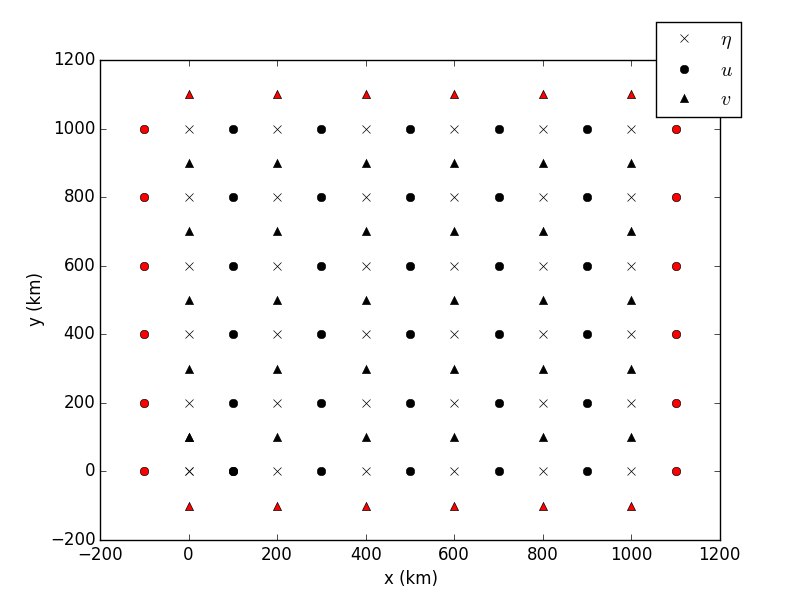
\includegraphics[width=300px]{figures/arakawa_c_grid}
    \caption{Shows where $\eta$, $u$ and $v$ are calculated on the Arakawa-C grid for $\Delta x =
	\Delta y = 250000\, m$ (lower than the lowest resolution used in this project, for
	illustration only). Note, $u$ is one bigger in the $x$ direction than $\eta$ (and similar
	for $v$ in $y$ direction), and therefore the minimum and maximum $u$ coordinates lie
	$\frac{\Delta x}{2}$ outside the domain (and similar for $v$). The red grid-point values
	show values which are held at $0$ due to the boundary conditions. }
    \label{fig:arakawa_c_grid}
\end{figure}

First $\eta$, $u$ then $v$ are calculated (in that order):

\begin{align}
    \label{eqn:swe_arakawa1} 
    \eta^{n+1} & =  \eta^n- H \Delta t (\frac{\partial u^n}{\partial x} + \frac{\partial v^n}{\partial y} ),  \\
    \label{eqn:swe_arakawa2} 
    u^{n+1} & = u^n + (f_0 + \beta y) \Delta t v^n - g \Delta t \frac{\partial \eta^{n+1}}{\partial
    x} - \gamma \Delta t u^n + \Delta t \frac{\tau_x}{\rho H}, \\
    \label{eqn:swe_arakawa3} 
    v^{n+1} & = v^n - (f_0 + \beta y) \Delta t u^{n+1} - g \Delta t \frac{\partial \eta^{n+1}}{\partial y} -
    \gamma \Delta t v^n + \Delta t \frac{\tau_y}{\rho H}.
\end{align}

Second $\eta$, $v$ then $u$ are calculated (note, the order of $u$ and $v$ calculations has been
swapped):

\begin{align}
    \label{eqn:swe_arakawa4} 
    \eta^{n+2} & =  \eta^{n+1}- H \Delta t (\frac{\partial u^{n+1}}{\partial x} + \frac{\partial
    v^{n+1}}{\partial y} ),  \\
    \label{eqn:swe_arakawa5} 
    v^{n+2} & = v^{n+1} - (f_0 + \beta y) \Delta t u^{n+1} - g \Delta t \frac{\partial \eta^{n+2}}{\partial y} -
    \gamma \Delta t v^{n+1} + \Delta t \frac{\tau_y}{\rho H}, \\
    \label{eqn:swe_arakawa6} 
    u^{n+2} & = u^{n+1} + (f_0 + \beta y) \Delta t v^{n+2} - g \Delta t \frac{\partial
	\eta^{n+1}}{\partial x} - \gamma \Delta t u^{n+1} + \Delta t \frac{\tau_x}{\rho H}.
\end{align}

To calculate $u$ on the other two grids (see \ref{fig:arakawa_c_grid}), spatial averging must
be used. E.g. to calculate $u$ on the $\eta$ grid, the average of two $u$ grid-points in the $x$
direction must be used, and to calculate $u$ on the $v$ grid, four grid-points in the $x$ and $y$
directions must be used. Similar calculations apply to $v$ and $\eta$ on the other grids.
Derivatives are calculated using the two values on either side of the grid-point where they are
needed (using the midpoint method which is 2nd order accurate, indeed this is the strength of the
Arakawa-C grid).

\section*{Task A}

To model the Western Boundary Current (WBC), a sufficient number of grid-points must span this
distance. If the size of the WBC is taken to be $\frac{1}{10}$ \ts{th} of the zonal extent of the
domain, or \SI{100}{km}, and four grid-points are required across this to capture its variation,
this would mean a minimum spatial resolution of $\Delta x = 25\, km$ should be used. In this Task, a
value of $\Delta x = \Delta y = 20\, km$ was used. Kinematic boundary conditions are used throughout
this study, i.e. $u$ is held at $0$ on the eastern and western boundaries, $v$ is held at $0$ on the
northern and southern boundaries.

The fastest signals propagating in this system are gravity-inertia waves. These have a phase speed
of $\sqrt{g H}$, and following XX Beckers\dots this can be used to calculate an upper bound for the
CFL criterion, i.e. $\sqrt{g H} \frac{\Delta t}{\Delta x} <= \frac{1}{4}$ will be a necessary
condition for the scheme to be stable. In practice, at the first resolution, it was found that the
less stringent requirement of $\sqrt{g H} \frac{\Delta t}{\Delta x} <= 1$ was necessary to ensure
numerical stability (from empirical experimentation). The first CFL criterion will be referred to as
the strict criterion, and the second the lax criterion. In light of this, in this task $\Delta t$ was
taken to be \SI{139}{s} so as to just satisfy this lax criterion. Satisfying the lax criterion
allows for a larger timestep and therefore less time is needed to run the simulations.

\begin{figure}[ht!]
    \centering
    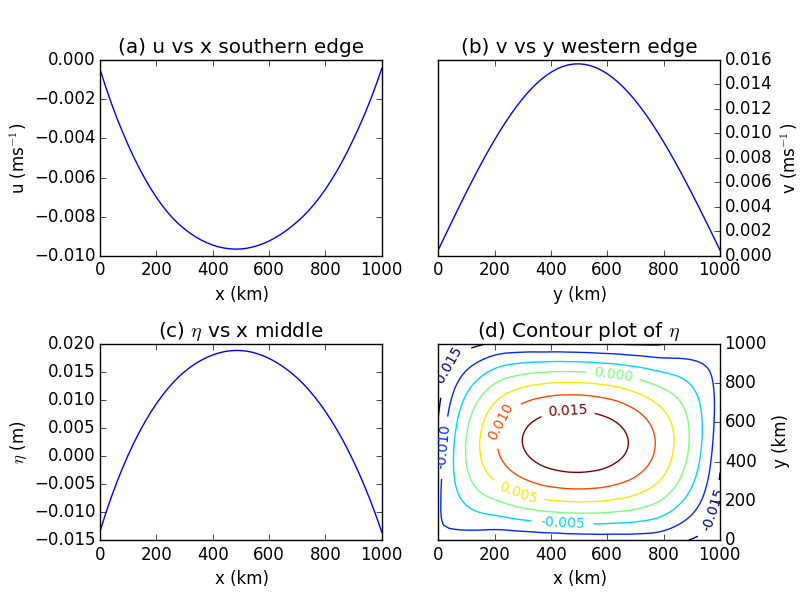
\includegraphics[width=300px]{figures/task_a}
    \caption{Four plots showing $u$, $v$ and $\eta$ along three different zonal/meridional extents
	after one day - (a), (b) and (c). Plot (d) shows $\eta$ over the whole domain after one
    day.}
    \label{fig:task_a}
\end{figure}
% Say something about Rossby radius of deformation and link to spatial resolution.
% Justify timestep/etc.

The model was run for one day, and various plots of $u$, $v$ and $\eta$ are shown in Figure
\ref{fig:task_a}. Overall, an anti-clockwise gyre is set up, as can be seen in plots (a) and (b)
because $u$ is negative along the southern boundary, and $v$ is positive along the western boundary.
Plot (d) shows that the height perturbation, $\eta$, is almost symmetrical after one day, although
anomalously high values can be seen in the northeast and southwest corners.

\section*{Task B}

The energy stored in the gyre can be calculated by summing the contributions from the kinetic energy
(terms one and two in the integrand in Equation \ref{eqn:energy}) and the gravitational potential
energy (term three):

\begin{equation}
    \label{eqn:energy} 
    E(u, v, \eta) = \int_0^L \int_0^L \frac{1}{2} \rho ( H ( u^2 + v^2) + g \eta^2) dx dy
\end{equation}

% TODO: CFL.
This can be approximated over the domain using Simpson's rule in 2D. This can then be calculated for
every timestep, as is shown in Figure \ref{fig:task_b_energy}. For this figure, the model was run at
two resolutions: once as before with $\Delta x = \Delta y = 10\, km$ , and once with $\Delta x =
\Delta y = 10\, km$ (i.e. twice the spatial resolution). A time step of $\Delta t = 30\, s$ was use
in both cases, so that the strict CFL criterion is still satisfied for the high resolution run and
that only changes in the spatial resolution are being compared between the two runs. (It was found
that running the model at the higher resolution with only the lax criterion being satisfied lead to
numerical instability after around \SI{50}{days}.) The model was run for 100 days in each case, and
it can be seen that the energy reaches a peak at around \SI{35}{days} before reducing by
2.05\%(1.26\%) for $\Delta x = 20$ \SI{}{km} ($\Delta x = 10$ \SI{}{km}) over the next
\SI{65}{days}.

\section*{Task C}

% Run these with same dt.
Given that the energy in the model is approximately constant after \SI{100}{days}, it can be
compared to the steady state analytical solution as found in (XXX Musgrave). The only unknown in
these equations is the value of $\eta_0$, for which the modelled value of $\eta(0, \frac{L}{2})$ is
used. One way of doing these comparisons is to work out the perturbations of $u$, $v$ and $\eta$ as
defined by e.g. $u' = u - u_{st}$, then calculating the energy difference using Equation
\ref{eqn:energy} - $E(u', v', \eta')$. Using this equation, when $\Delta x = 20$ \SI{}{km}, the
total energy difference between the analytical and the modelled steady state solution is
\SI{18.4}{TJ}, and when $\Delta x = 10$ \SI{}{km}, the total energy difference is \SI{4.98}{TJ}.
Therefore, increasing the resolution increases the accuracy of the modelled steady state solution.
The 2\ts{nd} order spatial accuracy of the 2D SWE numerical model on an Arakawa-C grid can be seen
from the fact that when the resolution is doubled, the error, as measured by the total energy
difference, is approximately four times smaller. 

\section*{Task C}

One way of solving a non-linear version of the SWE equations is to implement a semi-Lagrangian
numerical scheme. Here the full Lagrangian rates of change ($\frac{D}{Dt}$ as opposed to
$\frac{\partial}{\partial t}$) are used, and the departure point of each of each grid-point is
calculated to work out the previous value of $u$, $v$ and $\eta$ to be used. It is therefore
necessary to calculate the departure points for each of the $u$, $v$ and $\eta$ grids used in the
Arakawa-C grid.  To calculate the departure point, the $\boldsymbol{u} =  ($u$, $v$)$ field at two
previous timesteps is used. Following Durran pp366-368, first, a 2\ts{nd} order estimate for
$\boldsymbol{u}^{n + \frac{1}{2}}$ is calculated using $\boldsymbol{u}^{n + \frac{1}{2}} =
\frac{3}{2}  \boldsymbol{u}^{n} - \frac{1}{2} \boldsymbol{u}^{n-1}$. This is then used to calculate
a value of $\tilde{\boldsymbol{u}}$, the departure point, through the use of an intermediate
departure point using the following formulae:

\begin{align}
    \label{eqn:sl_update1} 
    \boldsymbol{x_{*}} = \boldsymbol{x}^{n+1} - \boldsymbol{u}(\boldsymbol{x}^{n+1}, t^n)
    \frac{\Delta t}{2},\\
    \label{eqn:sl_update2} 
    \boldsymbol{\tilde{x}}^n = \boldsymbol{x}^{n+1} - \boldsymbol{u}(\boldsymbol{x_{*}},
    t^{n+\frac{1}{2}}) \Delta t.\\
\end{align}

The departure points tell us where to take the values of $u$, $v$ and $\eta$ from in the previous
timestep. However, it is unlikely that these departure points will lie on grid-points, therefore it
is necessary to interpolate between the values of these three fields to calculate the values at the
departure points. This is achieved using the \lstinline[basicstyle=\ttfamily]|RectBivariateSpline|
class from the \lstinline[basicstyle=\ttfamily]|scipy.interpolate| namespace. By default this uses a
2D cubic spline interpolation, and this was used to implement the interpolation of the three fields
in this Task. It also gracefully handles the interpolation of points which are outside of its domain
by using the value of the nearest point in the domain of interpolation, which is useful for this
study. Once the departure points have been calculated for the three grids, the same forward-backward
time scheme used before is used to update the three fields. 


\begin{figure}[ht!]
    \centering
    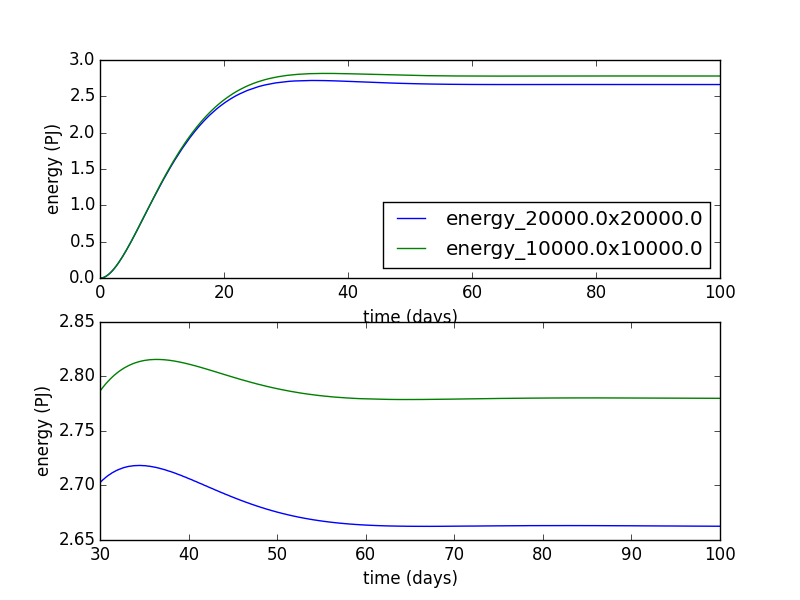
\includegraphics[width=300px]{figures/task_b_energy}
    \caption{The effect of spatial resolution on the total energy of the system. Doubling the
    spatial resolution (blue curve) increases the overall energy of the system. It also reduces the
energy difference between the analytical steady state solution and the steady state obtained by
running the SWE model for 100 days.}
    \label{fig:task_b_energy}
\end{figure}

\section*{Appendix A}

All code can be downloaded from the following link:

https://github.com/markmuetz/mtmw14

\end{document}

\end{document}
